\section{Implementierung}
\label{Implementierung}

\subsection{Messmodi}
\label{Messmodi}
In diesem Kapitel werden die implementierten Messmodi vorgestellt und die Herausforderungen der Umsetzung beschrieben. Zum Ende dieser Arbeit sind folgende Modi konfigurierbar:
\begin{itemize}
	\item 0: \ac{USB}-\ac{HID}-singleKey
	\item 1: \ac{USB}-\ac{HID}
	\item 2: \ac{CDC} (COM-Port)
	\item 3: \ac{BLE}-\ac{HID}
	\item 4: \ac{BLE}-\ac{HID}-singleKey
\end{itemize}
Sie werden in die Kapitel \ac{USB}-\ac{HID} und \ac{BLE}-\ac{HID} zusammengefasst und es wird auf den Modus \ac{BLE}-Windows-App eingegangen, der nicht umgesetzt wurde, jedoch für eine spätere Version geplant ist. Der Modus \ac{CDC} war zu Beginn dieser Arbeit bereits implementiert. \\
Zum Zeitpunkt der Implementierung der Dongle-App, war diese die oberste Abstraktionsschicht aller USB-Funktionalität. Das ist mit Einführung der Messmodi nicht mehr der Fall. Daher bedarf es einer neuen Abstraktionsschicht, die über der Dongle- und Fußschalterapp steht und deren verschiedenen Funktionalitäten dirigiert. Dadurch können die Operationsmodi programmatisch getrennt werden, sodass bestimmte Schritte der Initialisierung, wie das Einlesen der Konfigurationsdatei der zu verbindenden Geräte, in einem Modus wie \ac{HID} einzelnes Zeichen nicht ausgeführt werden. Außerdem bleibt die Anwendung dadurch leicht um neue Messmodi erweiterbar. 

\begin{figure}[H] 
	\centering
	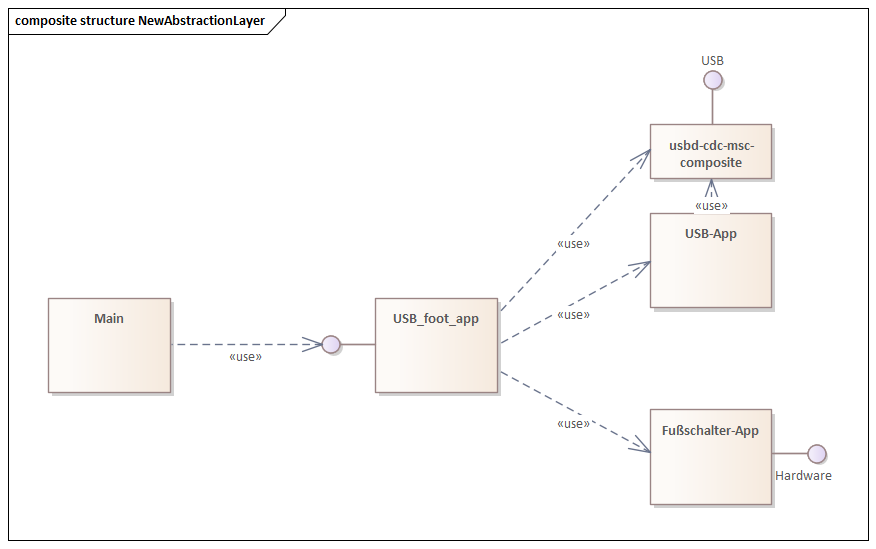
\includegraphics[width=\textwidth]{figures/NewAbstractionLayer.png}
	\caption{Neue Abstraktionsschicht}
\end{figure}

\subsubsection{USB-HID}
Ein Feature, das sowohl für den Dongle als auch für den Fußschalter implementiert werden soll, ist das Human Interface Device (HID) über USB. In diesem Modus gibt die Anwendung die Messergebnisse nicht mehr über den virtuellen COM-Port aus, sondern ist über USB als Tastatur mit dem Computer verbunden. Über sie werden die Zeichen der Messung als Tastendrücke, gefolgt von einem konfigurierbaren Terminierungszeichen, ausgegeben. Dadurch können Messungen in einem Tabellen Programm oder einem Texteditor aufgefangen werde.\\
Für die Implementierung werden die Funktionen des NRF-Library Files app\_usb\_hid\_kbd.h verwendet (\cite{NRF_USB_HID_keyboard}). Es abstrahiert die Low-Level USB-Aufrufe und stellt Funktionen zur Verfügung, die bei Aufruf eine Taste drücken oder loslassen. Es fehlt jedoch eine Funktion die ganze Strings serialisiert, weshalb diese implementiert werden muss. Die Scancodes, die Nummern der Tasturtasten, sowie der Modifier, eine Taste die Tastendrücke modifiziert, wie die Shift-Taste, werden dabei von einer Funktion erhalten, die im nrf\_Base Projekt enthalten ist. Sie wurde für die \ac{HID} Implementierung über \ac{BLE} geschrieben und gibt den Scancode und zugehörigen Modifier für einen \ac{ASCII} Character zurück.\\
Zwischen den Tastendrücken muss eine gewisse Zeit gewartet werden, da der Computer Tastendrücke zwischen denen zu wenig Zeit verstreicht nicht registriert. Dieser Delay wurde auf 1 Millisekunden festgelegt, was der maximalen Übertragungsrate über \ac{USB} entspricht (\cite[17]{HID_Specification}) und da bei einem längeren Delay die Anzahl an fehlerhaften Tastendrücken zunahm. Diese Art darauf zu warten, dass die Tastendrücke vom Computer registriert wurde, stellte sich jedoch als sehr fehleranfällig heraus. Nicht nur wurde dopplete Zeichen nicht korrekt erkannt, sondern nach ungefähr zehn Ausgaben schien der \ac{USB}-Bus überlastet zu sein und es erschienen keine Ausgaben mehr der Messergebnisse. Daher musste die Implementierung geändert werden. Statt die Tastendrücken ohne Rücksicht auf die zugehörigen Events dem \ac{USB} zu übergeben, muss nach jedem Zeichen auf ein Event der \ac{USB}-\ac{HID} Library gewartet werden, das die erfolgreiche Übertragung signalisiert. Dazu muss der zu serialisierende String in einem Buffer hinterlegt und bei Empfangen des Events das nächste Zeichen übertragen werden.\\
Eine Abwandlung dieses Modus, ist der Modus \ac{USB}-\ac{HID}-singleKey. In diesem Modus gibt der Fußschalter bei Betätigung des Tasters nur ein einzelnes kofigurierbares Zeichen aus, beziehungsweise bei einem Doppelklick ein Zweites, wie in Abschnitt \ref{UberarbeitungMSC} beschrieben ist.

\subsubsection{BLE-HID}
Ein weiterer Modus, in dem der Fußschalter arbeiten soll, ist \ac{HID} über \ac{BLE}. Dabei simuliert der Fußschalter oder Dongle eine über \ac{BLE} verbindbare Tastatur und serialisiert nach dem Verbinden wie bei \ac{HID} über \ac{USB} die Messergebnisse als Tastendrücken. Dazu muss das Gerät nun zusätzlich zur Central Rolle in der Peripheral Rolle agieren. Dazu muss einerseits das Advertising korrekt konfiguriert werden und in den bestehenden Code des Peripheren Verbindungsaufbaus, die Fußschalter Applikation eingebunden werden. Für das eigentliche Schreiben des Messergebnisses über \ac{BLE}, gibt es bereits eine bestehenden Funktionen des nrf\_Base Projekts die einen String vollständig serialisiert und diese muss nur in der Fußschalter Applikation aufgerufen werden.\\
Dabei erfordert dieser Modus es nun, dass die Bonding Informationen der Verbindung von Fußschalter zu Computer gelöscht werden kann. Werden sie nicht gelöscht, jedoch auf dem Computer, können sich die beiden Geräte nicht mehr miteinander verbinden. Das muss zum Beispiel geschehen, wenn der Fußschalter mit einem anderen Computer verbunden werden soll, sich der erste Computer jedoch noch in Reichweite befindet. Trotzdem sollen nicht bei jedem Reset des Fußschalter, also bei einer Änderung der Konfigurationsdatei, die Bonding Informationen gelöscht werden, da sonst bei jedem Verbinden, der Fußschalter im Computer erst entkoppelt und dann wieder neugekoppelt werden muss. Es kann also nicht direkt gesagt werden wann die Bonding Informationen gelöscht werden sollen und wann nicht, stattdessen wäre der Idealfall, dass der User selbst die Informationen löschen kann. Das ist jedoch aufgrund der begrenzten Interaktionsmöglichkeiten des Users mit dem Fußschalter nur schwierig umsetzbar. Ein Kompromiss ist, dass die Bonding Informationen gelöscht werden, wenn der Modus \ac{BLE}-\ac{HID} verlassen wird. Der Anwender kann dann auch um die Bonding Informationen zu löschen aus dem Modus 3 herauswechseln und dann wieder hineinwechseln. Dabei ist das Problem, dass bei einem Reset nicht direkt ersichtlich ist, in welchen Modus gewechselt wird, da die Konfigurationsdatei erst beim Neutstart neugelesen wird. Daher wird direkt vor dem Reset die Konfigurationsdatei gelesen und falls aus dem Modus 3 oder 4 in einen anderen Modus gewechselt wird, die Bonding Informationen gelöscht. Ein alternativer Lösungansatz der ohne das ressourcenfordernde Einlesen der Datei auskommt, ist die Bonding Informationen immer zu löschen, wenn sich der Fußschalter beim Reset in einem anderen Modus als 3 oder 4 befindet. Jedoch war dann der ``Peer Manager'' nicht initialisiert, der zum Löschen der Bonding Informationen zwingend benötigt wird, weshalb doch der erste Lösungansatz umgesetzt wurde. Der Peer Manager ist dabei eine Library von NRF die sich um Verschlüssung, Pairing und Bonding kümmert (\cite[]{NRF_PeerManager}).\\
Erste Tests zeigen, dass die Geschwindigkeit der Übertragung, einerseits die Dauer bis zum ersten Tastendruck und anderseits die Zeit zwischen den einzelnen Tastendrücken, zu hoch ist. Die Untersuchung wo genau zuviel Zeit verwendet wird, fand mithilfe eines Oszilloskop und dem togglen eines freien Pins, der zu diesen Debugzweck belegt wurde, statt. Es konnte dadurch bereits ein Bug im nrf\_Base Projekt gefunden werden. Dabei wird in der Funktion, zwischen den einzelnen Zeichen eine Pause gemacht, um ähnlich im Modus USB-\ac{HID} dem Betriebssystem Zeit zu geben die Tastendrücke zu verarbeiten. Dieser Delay ist abhängig von Connection Interval, welches wenn nur die Verbindung zum Computer besteht, korrekt gesetzt ist. Jedoch stellte sich heraus, dass diese globale Variable von allen Verbindungen stets überschrieben wird. Dabei ist diese Variable auch unabhängig von der \ac{HID} Funktionalität nur für die peripheren Verbindungen von Bedeutung und dieses Verhalten ein Fehler. Es wurde daher an der Stelle, an der diese Variable durch einen ``Connection Update Request'' überschrieben wird, die Unterscheidung eingeführt, ob es sich bei der Verbindung um eine periphere Verbindung handelt.\\
Auch von diesem Modus, gibt es die Abwandlung \ac{BLE}-\ac{HID}-singleKey, die wie im Modus USB-\ac{HID}-singleKey, ein einzelnes Zeichen bei Betätigung des Tasters ausgibt.


\subsubsection{BLE-Windows-App}
Der letzte Modus, in dem der Fußschalter agieren soll, ist als ein an die \ac{HCT}-Windows-App angebundenes Gerät. Dabei soll das Signal der Betätigung des Tasters als eine \ac{HCT}-Nachricht an die Windows-App gesendet werden, welchen dann ein Messergebnis bei den mit ihr verbundenen Messgeräten triggert. Dazu muss ein \ac{HCT}-Model für den Fußschalter geschaffen werden. Das Model stellt folgende Werte bereit:
\begin{itemize}
	\item Device Class
	\item Protocol type, version 
	\item Version of Hardware, Software, \ac{BLE}
	\item Battery level, status
	\item Reset 
\end{itemize}

Werte des Config.ini Konfigurationsfiles:
\begin{itemize}
	\item Operating Mode 
	\item \ac{CDC} protocol 
	\item HID Keyboard Language ID 
	\item HID data set seperator 
	\item HID number seperator
	\item HID single key single press
	\item HID single key double press
	\item Inactivity timeout
	\item sequentiel group triggering 
\end{itemize}

Für die Übertragung des eigentlichen Signals, dass der Fußschalter betätigt wurde, muss eine \ac{HCT}-Charakteristik angelegt werden, auf welche die \ac{HCT}-Windows-App sich subscriben kann. Über diese Charakteristik wird sie dann über die Betätigung des Tasters notifiziert. Im Advertising muss sich der Fußschalter dann nicht als Tastatur, sondern als \ac{HCT}-Fußschalter erkenntlich zeigen.\\
Es wurde jedoch beschlossen, diesen Modus erst in einer späteren Version des Fußschalters zu implementieren, wie im Abschnitt 8.2 genauer erklärt wird.

\subsection{Überarbeitung des MSC}
\label{UberarbeitungMSC}
In diesem Kapitel wird gezeigt durch welche Schritte die finale Lösung zur Detektion einer Änderung der Konfigurationsdateien erarbeitet wurde.

\subsubsection{Evaluierung der Möglichkeiten zur Detektion}
Der erste Versuch der unternommen wurde um dem Anwendungsfall gerecht zu werden, ist über die File Information des \ac{FAT} Filesystems den Änderungszeitpunkt auslesen und falls er sich im Vergleich zum Zeitpunkt, der beim erstmaligen Einlesen festgestellt wurde, geändert hat, ein Systemneustart durchzuführen. Dabei hat sich jedoch gezeigt, dass eine Änderung an der Datei keine Veränderung am Änderungszeitpunkt hervorruft. Erst nach einem manuellen Reset zeigt sich das korrekte Änderungsdatum in der File Information. \\
Ein weiterer Versuch war es, direkt zu überprüfen ob neue Daten über das Blockdevice geschrieben wurden. Das Blockdevice ist dabei eine Zwischenschicht zwischen Filesystem und dem physischen Speicher(\cite{NRF_Block_device}). Das führte jedoch dazu, dass der Systemneustart durchgeführt wurde, bevor alle Daten vollständig geschrieben wurden. Zudem hat diese Implementierung weitere Probleme, wie zum Beispiel, dass ein Formatieren des Datenträgers, wie er bei der ersten Inbetriebnahme durchgeführt werden muss, nicht mehr möglich war. \\
Ein periodisches Neueinlesen der Daten war hingegen nicht möglich, weil beim Lesen der Daten die Anwendung in einer Warteschleife festhing. Es zeigte sich, dass sowohl \ac{MSC} als auch das \ac{FAT} Filesystem auf die gleiche Instanz des Blockdevice versucht haben zuzugreifen, was grundsätzlich nicht möglich ist. Ein Anlegen einer weiteren Instanz des Blockdevice für das Filesystem behob dieses Problem. \\
In einer zwischenzeitlichen Lösung des Problems werden die Konfigurationsfiles periodisch neugelesen und über die Daten ein Hashwert gebildet. Anhand dieses Wertes wird dann eine Änderung festgestellt. Hat sich das globale Konfigurationsfile geändert wird ein Systemreset durchgeführt, während bei einer Änderung des Files der zu verbindenden Geräte, die Verbindung zu allen Geräten getrennt wird und das File anschließend neueingelesen, wodurch der Verbindungsaufbauprozess neu gestartet wird. Jedoch zeigte sich, dass Änderungen, die am Ende der Datei stattgefunden haben, nicht detektiert werden. Durch genaue Analyse des Prozess konnte festgestellt werden, dass die Länge der Datei nicht erneut eingelesen wird, wenn die Datei aus dem Massenspeichermedium heraus geändert wurde und nicht aus dem Filesystem auf dem Chip. Daher können Änderungen an den Dateien, die ausschließlich hinten an dem bestehenden Text angefügt werden, nicht detektiert werden, da die Datei mit der alten Länge eingelesen wird.

\subsubsection{Manuelles Einlesen des Änderungszeitpunkts}
Es konnte festgestellt werden, dass die Information, wie lang die Konfigurationsdatei ist, korrekt im Speicher vorhanden ist, aber nicht ins interne Filesystem übernommen wird. Es besteht also die Möglichkeit die Informationen selbstständig einzulesen. Dazu muss als Erstes das ``Directory Entry'' gefunden werden. Es steht nach den \ac{FAT} und beeinhaltet Informationen zur Datei, wie die Länge in Bytes und das Änderungsdatum (\cite[Abschnitt 1.4]{FAT}). Daher müssen folgende Informationen aus der Boot Section ausgelesen werden und folgende Berechnung durchgeführt werden:
\begin{itemize}
    \item Sa: Startadresse Filesystem
    \item Sg: Sektorengröße
    \item nrS: Anzahl reservierter Sektoren
    \item nF: Anzahl \ac{FAT}
    \item nSF: Anzahl Sektoren pro \ac{FAT}
\end{itemize}

\[Sa + Sg \cdot nrS + Sg \cdot nF \cdot nSF = Sa + Sg\cdot(nrS + nF \cdot nSF)\]

Diese Informationen stehen jedoch immer an der gleichen Stelle im Bootsektor und ändern sich während des Betriebs des Fußschalters nicht. \\
Im Directory Entry wird jeweils für die Informationen einer Datei 32 Bytes verwendet und innerhalb dieser 32 Bytes befinden sich die Informationen immer an der gleichen Stelle, weshalb mit festen Offsets gearbeitet werden kann. Jedoch wird ein Eintrag nicht sofort gelöscht, wenn die Datei gelöscht wird, sondern die Filenamen durch Ersetzten des ersten Buchstaben durch 0x5a invalidiert (\cite[Abschnitt 1.4]{FAT}). Daher muss der valide Eintrag immer wieder neu gesucht werden. Dadurch kann das Directory Entry größer als ein Sektor werden, auch wenn er nur zwei Dateinamen beeinhaltet. Es wird daher nacheinander die Sektoren, die für das Directory Entry allokiert sind, eingelesen und auf die korrekten Dateinamen hin untersucht. Ist der korrekte Eintrag gefunden, wird der Änderungszeitpunkt eingelesen und nach der bereits beschriebenen Methode überprüft. Es wurde hier wieder der Änderungszeitpunkt zur Detektion einer Änderung verwendet, da die Länge der Datei nur dazu benutzt werden könnte, die Datei ``händisch'' einzulesen, also direkt über Flash Zugriffe und nicht über die \ac{FAT} Filesystem Library. Was kurzzeitig in Angesicht der weiterhin bestehenden Probleme in Erwägung gezogen wurde, aber aufgrund des hohen Entwicklungsaufwands versucht wurde zu vermeiden. Dabei kann aus dem Directory Entry auch der Startsektor der Datei ausgelesen werden und ähnlich der Adresse des Directory Entry, die Adresse des Sektors berechnet werden. Auf den ersten Blick erscheint das nicht übermäßig kompliziert, jedoch wird die Datei, falls sie größer als ein Sektor wird, auf nicht zwangsläufig aufeinanderfolgende Sektoren verteilt, was nur anhand der \ac{FAT} nachvollzogen werden kann.

\subsubsection{Finale Lösung}
Das Hauptproblem des \ac{MSC} ist, dass es immer wieder dazu kommt, dass Schreibbefehle fehlschlagen und die Daten unvollständig in den Speicher übertragen werden. Dabei wurde davon ausgegangen, dass die Schreibbefehle fehlschlagen aufgrund, weil der Neustart des Fußschalters zu früh erfolgt und die zu schreibenden Daten nicht vollständig in den Speicher übertragen wurden. Schließlich zeigte sich das als eine grundlegende Fehlannahme und stattdessen ergeben Nachforschungen, dass die Zugriffe auf den Flash vom Softdevice abgearbeitet werden müssen und dass aufgrund mehrere aktive Verbindungen die Wahrscheinlichkeit von Fehlerhaften Schreibzugriffen stark ansteigt (\cite[Abschnitt SoftDevice Backend]{NRF_fstorage}). Getätigte Änderungen an den Konfigurationsfiles werden dann nicht übernommen und sind selbst nach langen Wartenzeiten, nach dem Reset verloren. Deshalb werden, falls Schreibzugriffe gequeuet sind, alle Aktivitäten des Softdevice gestoppt, um die Gefahr von Fehlern beim Schreiben und die benötigte Zeit zu minimieren. Das umfasst das Trennen aller Verbindungen, sowie das Stoppen von Advertising und Scanning. Da durch einen gestarteten Timer der Fußschalter ohnehin neugestartet werden soll, damit die Konfigurationsfile neueingelesen werden können, ist die Beeinträchtigung der User Experience vernachlässigbar.\\
Diese Problematik besteht auch im Modus \ac{BLE}-\ac{HID}, da die Bonding Informationen über die selbe Library vom Softdevice in den Flash geschrieben werden (\cite{NRF_PeerManager}). Hat sich der Fußschalter zum Zeitpunkt des Verbindens mit dem Computer bereits mit mehreren Werkzeugen verbunden, besteht eine hohe Wahrscheinlichkeit, dass die Bonding Informationen fehlerhaft geschrieben werden. Der Fußschalter kann sich dann nicht mehr mit dem Computer verbinden beziehungsweise kann keine Zeichen bei einer bestehenden Verbindung übertragen. Die Lösung dieses Problems besteht darin, das Verbinden des Werkzeugs erst zu starten, wenn die periphere Verbindung zum Computer, bereits besteht. Da ohne die Verbindung zum Computer dieser Modus nicht nutzbar ist, ist die Userexperience dadurch nicht beeinträchtigt.

\subsection{Einbindung Messuhren}
\label{EinbindungMessuhren}
In Vorbereitung auf die Implementierung der fußschalterspezifischen Features wird die Dongle-App um die Unterstützung der Messuhren bzw. Messschieber erweitert, da sich die meiste Funktionalität des Fußschalters speziell auf die Messuhren bezieht. Messuhren und Messschieber sind in diesem Kontext dabei gleich bedeutend, weil das \ac{HCT}-Interface für beide Geräte identisch ist. Es wird sich nachfolgend jedoch stets auf Messuhren bezogen, da sie für die Anwendungsfälle des Fußschalters und Dongles bedeutender sind.

\subsubsection{Unterscheidung der Geräte}
Im einfachsten Anwendungsfall ist der Fußschalter mit mehren Werkzeugen verbunden und sammelt passiven deren Messergebnisse auf. Unabhängig vom eingestellten Messmodus benötigt die Dongle-App von den Geräten einerseits das Messergebnis und andererseits die Messeinheit, um die Ergebnisse vollständig an den Computer weitergeben zu können. Diese befinden sich abhängig vom Gerät an folgenden \ac{HCT}-Protokoll-Adressen:

\begin{table}[H]
	\centering
	\begin{tabular}[H]{l|l|l}
		 & Datenblock & Adresse \\
		\hline
		Garant Drehmomentschlüssel & & \\
		Messergebnis & Measurement data block & 0x00000B04 \\
		Messeinheit & Setpoint data block & 0x00000C1F \\
		\hline
		Holex Drehmomentschlüssel & & \\
		Messergebnis & Device measurement result & 0x0000240C \\
		Messeinheit & Device measurement case config & 0x0000221B \\
		\hline
		Messuhren/Messschieber & & \\
		Messergebnis & Device measurement result & 0x00002408 \\
		Messeinheit & Device measurement case config & 0x0000220F \\
		
	\end{tabular}
	\caption{Adressen Messergebnis und Messeinheit}
\end{table}

In Tabelle 1 wird deutlich, dass die Adressen von Messergebnis und Messeinheit für diese drei Geräte jeweils unterschiedlich sind, auch wenn sie im Fall der Messuhren und Holex Drehmomentschlüssel im gleichen Datenblock liegen. Wird dieser als Binärdaten erhalten kann die Adresse des Datenblocks gelesen werden, die Information von welchem Gerät die Daten stammen und damit an welcher Stelle genau die jeweils die Daten zu finden sind, kann jedoch nicht festgestellt werden. Es bleibt also keine andere Möglichkeit als die verbundenen Geräte ihrem Typ zuzuordnen und die erhaltenen Daten entsprechend zu interpretieren.\\ 
Diese Unterscheidung mit welcher Art von Gerät kommuniziert wird, kann auf zwei verschiedenen Weisen erfolgen. Einerseits kann anhand des Namens das Gerät entweder der Klasse Drehmomentschlüssel oder Messuhr zugeordnet werden. Das ist jedoch unter Umständen fehleranfällig, da das Sortiment an \ac{HCT}-Werkzeug stetig wächst und es nicht auszuschließen ist, dass in der Zukunft Geräte auf den Markt kommen, mit deren Namen es zu falschen Zuordnung kommt. Zudem gibt es alte Messschieber, die zwar unter einem korrekten Name advertisen aber nicht das \ac{HCT}-Protokoll sprechen, wobei diese Geräte aufgrund der Inkompatibilität der Protokolle letztendlich nicht verbunden werden sollten.\\
Eine andere Methode ist, die ``Device Information'' abzufragen und anhand der Klassenidentifikationsnummer das Gerät einem Typ zuzuordnen. Das ist die präferierte Lösung, da neben der genaueren und sicheren Zuordnung, in der Device Information andere Informationen, wie die Protokoll Version mitgeliefert werden, die bei späteren Features unter Umständen benötigt werden. Zudem bleibt die Datenverarbeitung leichter erweiterbar um neue Geräte. Jedoch muss diese Abfrage in den asynchronen und mehrteiligen Ablauf des Verbindungsaufbaus eingefügt werden, wodurch ein höherer Entwicklungsaufwand entsteht. Auch benutzen Drehmomentschlüssel der Firma Garant eine andere Klassifikation der Geräte als das Werkzeug der Firma Holex, welche innerhalb der Dongle-App vereinheitlicht werden muss.\\
Da die Erweiterbarkeit und Flexibilität jedoch dem höheren Entwicklungsaufwands überwiegen, wurde sich zugunsten dieser Lösung entschieden. Dabei wird nach dem Verbindungszustand-Callback, der vom Central Device nach einer erfolgreichen Subscription der Anwendung auf die \ac{BLE}-Charakteristik des Werkzeugs aufgerufen wird, eine Nachricht zu Abfrage der Device Information gesandt. Die erhaltenen Daten werden dann in der zum Gerät gehörenden Struktur gespeichert und anschließend die Abfrage der Messeinheit durchgeführt. 

\subsubsection{Anpassung der Messdatenverarbeitung}
Auch die Datenverarbeitung, also die Interpretation der erhalten Daten über \ac{BLE} muss angepasst werden, da das Messergebnis, wie bereits in Tabelle 1 gezeigt, zwar innerhalb des gleichen Datenblocks wie bei dem Holex Drehmomentschlüssel liegt, jedoch innerhalb des Datenblocks an einer anderen Stelle. Diese Offsets sind als Konstanten im Headerfile der Dongle-App definiert und müssen um die entsprechenden Einträge für die Messuhren erweitert werden. Werden die Daten erhalten, wird als Erstes die Adresse ausgelesen und dann je nach Typ des zugehörigen Geräts, die Interpretierung der Daten durchgeführt. Sollen also weitere Geräte eingebunden werden, können zusätzliche Sonderbehandlungen der Daten anhand des Typs hinzugefügt werden. Zudem handelt es sich bei dem Messergebnis, das von Interesse ist, beim Drehmomentschlüssel um den ``Peak Torque'', der als Gleitkommazahl codiert ist, während bei der Messuhr das Ergebnis die ``Measurement Distance'' als Ganzzahl codiert ist. Dabei handelt es sich abhängig von der Messeinheit um Mikrometer oder Mikroinch. Es muss auf Millimeter beziehungsweise Inch umgerechnet werden, da die Ausgabe über \ac{CDC} oder \ac{HID} der Anzeige auf dem Gerätedisplay gleichen soll. Das binäre Messergebnis wird daher zunächst mit einem Umrechnungsfaktor von 1000 in Millimeter beziehungsweise Milliinch als Gleitkommazahl umgerechnet. Anschließend muss überprüft werden, ob es sich bei der derzeitige Einheit des Geräts um Inch handelt, da dann der Wert erneut durch 1000 dividiert werden muss, um von Milliinch auf die gewünschte Einheit Inch zu gelangen. Es wird also letztendlich eine Gleitkommazahl erhalten, wodurch sie ohne Anpassungen in der Nachrichten Struktur der Dongle-App gespeichert werden kann.\\
Die Einheitenkodierung der Messuhr ist komplementär zur Kodierung der Drehmomentschlüssel und daher kann die if-Cascade, welche die Zuordnung vornimmt, um die Einheiten der Messuhr erweitert werden. Jedoch befindet sich die Information welche Einheit verwendet wird, wie das Messergebnis, ebenfalls an einer anderen Stelle innerhalb des Datenblocks und muss entsprechend angepasst werden.

\subsubsection{Gruppenfunktion}
\label{Gruppenfunktion}
Durch das Betätigen des Fußtasters des Fußschalters soll bei allen verbundenen Messuhren das derzeitige Messergebnis abgefragt werden. Während im Modus 2 (\ac{CDC}) ein Messergebnisse, anhand der Kanalnummer einem Werkzeug zugeordnet werden kann, ist dies in den \ac{HID}-Modi nicht der Fall. Es muss daher die korrekte Reihenfolge der Ausgabe der Messergebnisse sichergestellt werden. Es wurde sich entschieden, das devices.csv Konfigurationsfile um eine Spalte mit einer Gruppennummer zu erweitern, da somit der Anwender sowohl die Reihenfolge als auch welche Messuhren in der Gruppe sind, konfigurieren kann. Da durch das Abschicken der Nachrichten zur Abfrage der Messungen in der korrekten Reihenfolgen, das tatsächliche Erhalten in der gleichen Reihenfolge nicht sichergestellt ist, muss davon ausgegangen werden, dass die Nachrichten in einer zufälligen Reihenfolgen erhalten werden. Stattdessen muss bei der Ausgabe die Nachrichten umsortiert werden. Dazu bedarf es eines Zählers, der durch Betätigung des Fußschalters, von 0 auf 1 gesetzt wird, wodurch der Start der Gruppenfunktion später beim Erhalten der Messergebnisse erkennbar ist. Bei der Abarbeitung der erhaltenen Nachrichten, wird dann über die Zuordnung zum Device, die Nachricht ausgewählt und weitergegeben, die zum Counter korrespondiert. Die Gruppenids, die keinem der konfigurierten Geräte zugeordnet werden können, sowie die Gruppenids die zu unverbundenen Geräten gehören, werden dabei übersprungen. Zusätzlich soll ein Feature der Messeruhren genutzt werden, um die Gruppennummer auch auf der Messuhr anzuzeigen. Dazu werden den Messuhren ihre Gruppennummer nach dem Verbindungsaufbau via dem \ac{HCT}-Protokoll übermittelt.\\
Durch spätere Anregungen von Messtechnikern, die für den Vertrieb von Messwerkzeug zuständig sind, ergab sich jedoch, dass wenn ein Gerät der Gruppe zwar konfiguriert, jedoch nicht verbunden ist, die präferierte Lösung ist die gesamte Gruppe nicht zu triggern. Das ergibt sich einerseits dadurch, dass die Messuhren sich aufgrund ihrer relativ kleine Batterien bei Inaktivität schnell ausschalten und die Verbindung zu ihrem Central trennen. Anderseits soll möglichst jede durchgeführte Messung korrekt sein, da sie durch die \ac{CAQ}-Software verarbeitet und gespeichert wird. Das Ziel der Sicherstellung einer korrekten Messung überwiegt hier also dem Gedanken der Benutzerfreundlichkeit, dass eine Messung auch dann gemacht werden kann, wenn einer der Geräte unverbunden ist. Der Fußschalter blinkt dann zwei Mal kurz rot auf, um diesen Fehler zu signalisieren.\\
Des Weiteren könnte es passieren, dass eine Messung zwar angefragt, aber nicht erhalten wurde. Die Anwendung würde dann blockieren, da auf die Nachricht gewartet wird und müsste neugestartet werden. Es wurde sich entschieden, einen Timer zu starten, falls eine Nachricht nicht erhalten wurde und bei seinem Ablaufen statt dem Messergebnis eine Fehlermeldung auszugeben. Die restlichen Messergebnisse können dann korrekt ausgegeben werden.\\
Ebenfalls aus dem Feedback der Messtechnikern heraus, wurde ein sequentielles Triggern der Gruppe implementiert. Dazu muss der entsprechende Eintrag in der Konfigurationsdatei mit einer Eins auf aktiv gesetzt werden. Es wird bei den Geräten der Gruppe nacheinander, jeweils bei Betätigen des Fußtaster, die Abfrage eines Messergebnis ausgegelöst.

\subsection{Einbindung Hardware}
\label{EinbindungHardware}
Die Prototypen des Fußschalters der Firma Brecht wurden bereits vor Beginn dieser Arbeit erhalten und somit konnte direkt mit der Inbetriebnahme der neuen Hardware begonnen werden. Der Chipsatz des Fußschalters ist ebenfalls der PCA10056 von Nordic semiconductor, somit muss an der Software des \ac{USB}-Dongles keine Änderungen vorgenommen werden. In diesem Kapitel werden die hardwarebezogenen Funktionalitäten des Energiemanagements, des Fußtaster und der \ac{LED} vorgestellt. Im Anhang finden sich die ursprünglichen Hardwarezeichnungen der Platine.

\subsubsection{Energie Management}
Um den Fußschalter herunterzufahren und den Stromverbrauch zu senken, sah eine erste Idee vor das im nrf\_Base Projekt vorhandene Energiemanagement zu benutzen. Dieses fährt aus dem Main-Loop heraus getriggert den Chip bei Inaktivität des Softdevice weitestgehend herunter, wodurch der Stromverbrauch stark sinkt. Ist der \ac{USB}-Port also nicht verbunden und es wurde keine Aktivität in der Fußschalter Anwendung registriert, wird ein Timer gestartet. Läuft dieser Timer ab, werden alle \ac{BLE}-Verbindungen getrennt und falls notwendig Scanning und Advertising gestoppt. Wird während dem Laufen des Timers Aktivität registriert, wird er neugestartet, während er vollständig gestoppt wird, falls \ac{USB} wieder verbunden ist. Dieser Implementierung lag die Vermutung zugrunde, dass wenn der Chip vollständig heruntergefahren wurde, er auch nicht durch Betätigung des Fußtasters wieder neugestartet werden kann.\\
Zunächst zeigte sich jedoch das Problem, dass bei der Hardware des Fußschalters, der Akku auf der Datenleitung des \ac{USB} liegt. Dadurch wird in der Anwendung nicht wie bei dem EvalBoard die Events für \ac{USB} connected und \ac{USB} disconnect erhalten. Daher musste am Fußschalter geringfügige Hardwareänderungen durchgeführt werden. Dabei wurde die Eingangsspannung bereits vorher abgegriffen und auf den Pin des Fußtasters gelegt. Der Fußtaster erhält einen unbelegten Pin. Mit einem \ac{ADC} wird dann überprüft, ob eine Spannung auf diesem Pin anliegt.\\
Es zeigte sich bei der Einbindung des Fußtasters, dass die Anwendung durch Betätigung des Fußtasters selbst aus einem Shutdown heraus wieder aufgeweckt wird. Daher wird nach Ablaufen des Inaktivitätstimers die Anwendung vollständig heruntergefahren, was noch energieeffizienter ist.

\subsubsection{Fußtaster Funktionalität}
Nach Überarbeitung der Codebasis und Einbindung der Messuhren, stehen alle Funktionalitäten bereit um den eigentlichen Fußtaster einzubinden. Während bei der initialen Einbindung des Fußtasters, eine Betätigung das Abfragen der Messergebnisse bei allen verbundenen Messuhren triggerte, wuchs die Funktionalität stetig.\\
Zum Ende dieser Arbeit wird durch ein kurzes Betätigen oder einem ``einfachen Klick'' die bereits beschriebene Gruppenfunktion ausgeführt. Im Modus 0 (USB-\ac{HID}-singleKey) und 4 (\ac{BLE}-\ac{HID}-singleKey) wird draufhin ein Timer gestartet, welcher derzeit auf 500ms gesetzt ist. Wird während seines Laufen eine zweite Betätigung getätigt, wird ein ``Doppelklick'' registriert und das dafür in der Konfigurationsdatei hinterlegte Zeichen ausgegeben. Dadurch kann der User in diesem Modus schnell Dialogoptionen in der \ac{HCT}-Windows-App auswählen oder in einem Textfile die Seiten wechseln. In einem anderen Modus führt das Warten auf die zweite Betätigung, jedoch zu einer Verzögerung der Ausgabe um die Dauer des Timers, weshalb dort die Doppelklick Funktionalität zugunsten des Ansprechverhalten des Tasters gestrichen wurde.\\
Wird der Taster hingegen für 3 Sekunden durchgängig gehalten, wird das Gerät heruntergefahren. Diese Funktionalität wurde ursprünglich eingeführt, da der Fußschalter auf einer Messe vorgestellt wurde, aber der automatische Reset des Geräts bei Änderung der Konfigurationsfiles noch nicht implementiert war. Sie wurde aufgrund von positiven Feedback beibehalten.

\subsubsection{Inbetriebnahme LED}
Auf dem Board des Fußschalters befindet sich eine \ac{LED} die durch einen Lichtkanal nach außen hin durch das Gehäuse sichtbar gemacht wird und die dazu benutzt werden soll den internen Zustand des Geräts darzustellen. Folgende Zustände sollen abgebildet werden: 

\begin{table}[H]
	\centering
	\begin{tabular}[H]{l|l}
		Zustand & \ac{LED}-Farbe \\
		\hline
		Gerät im Sleep Modus & Aus \\
		\hline
		Alle zu verbindenden Geräte verbunden & Blau \\
		\hline
		Min. ein Gerät verbunden, es wird nach den fehlenden Geräten gescannt & Blau blinkend \\
		\hline
		Kein Gerät verbunden, Scanning inaktiv & Grün \\
		\hline
		Kein Gerät verbunden, Scanning aktiv & Grün blinkend \\
		\hline
		\ac{MSC}-Schreibvorgang detektiert & Gelb \\
		\hline
		Min. ein Konfigurationsfile nicht gefunden & Rot \\
		\hline
		Fehler in den Konfigurationsfiles & Rot blinkend \\
	\end{tabular}
	\caption{LED-Zustände}
\end{table}

Zudem blinkt der Fußschalter, wie in Kapitel \ref{Gruppenfunktion} beschrieben, zwei mal kurz rot auf, wenn bei Betätigung des Fußtasters nicht alle zu der Gruppe gehörenden Geräte verbunden sind. Außerdem blinkt die Drei-Farben-\ac{LED} des Fußschalters vor einem Neustart oder dem Ausschalten des Geräts zweimal kurz grün.
